%@ autor Damien Meur
\documentclass{article}[12pt]

%--------------Packages------------------------------
\usepackage[utf8]{inputenc} %Pour encoder du texte en français
\usepackage[francais]{babel} %Pour encoder du texte en français
\usepackage{graphicx} %pour inclure des images
\usepackage{version} % permet d'utiliser l'environnement comment
\graphicspath{{./figures/}} %repertoire images
\usepackage{listings} %si on veut afficher du code, le code doit se trouver dans un dossier "codes" 					  %lui même dans le même répertoire que ce fichier tex
\usepackage{color} %nécessaire pour changer les couleurs du highlighting du code
\usepackage{amsmath,amssymb}%pour des maths au cas où
\usepackage{array,multirow,makecell}%Pour manipuler les tableaux
\usepackage{url} %pour utiliser les liens hypertextes
\usepackage{hyperref} %pour utiliser les liens hypertextes
\usepackage{float}

\newlength{\length}
\setlength{\length}{3\baselineskip}

%---------------Liste macros utiles------------------
\begin{comment}

%1.Inclure une image
\begin{figure}[!h]
\center
\fbox{\includegraphics[width=5cm,height=5cm]{figure1.jpg}}
\caption{Superbe image}
\end{figure}

%2. Inclure un tableau
\begin{table}[!h]
    \center
    \begin{tabular}[b]{|l|c|c|c|}
    \hline
    & \multicolumn{3}{|c|}{Année} \\
    \hline
    Produit & 1999 & 2000 & 2001 \\
    \hline \hline
    Livre & 15 & 10 & 7 \\
    CD & 10 & 17 & 22 \\
    \hline
    \end{tabular}
    \caption{Vente pour les années 1999 à 2001}
\end{table}

%3. Inclure une (ou des) définitions
\begin{description}
  \item[Premier] Le premier élément
  \item[Deuxième] Le deuxième élément
  \item[Troisième] Le troisième élément
\end{description}

%4. Inclure une bibliographie
\begin{thebibliography}{1}
    \bibitem{latexpratique} Christian \textsc{Rolland}. \emph{\LaTeX{} par la pratique}. O'Reilly, 1999.
\end{thebibliography}

%5. Inclure une note de bas de page
\footnote{On a ici inséré une espace normale}

%remarque 1  on peut faire référence à une entrée de la bibliographie en bas de page grâce à:
\cite{latexpratique}

%remarque 2  on peut faire des référence grâce à :
\label{distances} % dans le tableau ou l'environnement  à rérérencer
\ref{distances} %pour référencer

%6. Inclure  du code (ici Java) (avant \begin{document})
\definecolor{dkgreen}{rgb}{0,0.6,0}
\definecolor{gray}{rgb}{0.5,0.5,0.5}
\definecolor{mauve}{rgb}{0.58,0,0.82}
\lstloadlanguages{Java}

\lstset{frame=tb,
  %inputpath={./codes/},
  language=Java,
  aboveskip=3mm,
  belowskip=3mm,
  showstringspaces=false,
  columns=flexible,
  basicstyle={\small\ttfamily},
  numbers=none,
  numberstyle=\tiny\color{gray},
  keywordstyle=\color{blue},
  commentstyle=\color{dkgreen},
  stringstyle=\color{mauve},
  breaklines=true,
  breakatwhitespace=true,
  tabsize=3
}
%la macro a utilisé
\newcommand{\JAVAcode}[2]{
\begin{itemize}
\item[]\lstinputlisting[caption=#2,label=#1]{#1.java}
\end{itemize}
}
%on l'emploie de cette manière dans le texte (premier parametre est le nom du fichier, le second est %le caption
\JAVAcode{F5D1}{Exemple de code java}

%7. passer plusieurs lignes
\vspace{1\baselineskip}


\end{comment}
%-------------------------------------------------------------------

\begin{document}


\begin{titlepage}

\newcommand{\HRule}{\rule{\linewidth}{0.5mm}} % Defines a new command for the horizontal lines, change thickness here

\center % Center everything on the page
 
%----------------------------------------------------------------------------------------
%	HEADING SECTIONS
%----------------------------------------------------------------------------------------

\textsc{\LARGE Institut Paul Lambin}\\[1.5cm] % Name of your university/college
\textsc{\Large BAC 2 Informatique de gestion}\\[0.5cm] % Major heading such as course name
\textsc{\large Cahier des charges}\\[0.5cm] % Minor heading such as course title

%----------------------------------------------------------------------------------------
%	TITLE SECTION
%----------------------------------------------------------------------------------------

\HRule \\[0.4cm]
{ \huge \bfseries Outil de gestion des bugs et des demandes d'améliorations }\\[0.4cm] % Title of your document
\HRule \\[1.5cm]
 
%----------------------------------------------------------------------------------------
%	AUTHOR SECTION
%----------------------------------------------------------------------------------------

\begin{minipage}{0.4\textwidth}
\begin{flushleft} \large
\emph{Auteurs:}\\
Christopher \textsc{Sacré} \\
Antoine \textsc{Maniet} \\
Alexandre \textsc{Maniet} \\
Timothé \textsc{Bouvin} \\
Damien \textsc{Meur} % Your name
\end{flushleft}
\end{minipage}
~
\begin{minipage}{0.4\textwidth}
\begin{flushright} \large
\emph{Professeur:} \\
B. \textsc{Lehmann} % Supervisor's Name
\end{flushright}
\end{minipage}\\[4cm]

% If you don't want a supervisor, uncomment the two lines below and remove the section above
%\Large \emph{Author:}\\
%John \textsc{Smith}\\[3cm] % Your name

%----------------------------------------------------------------------------------------
%	DATE SECTION
%----------------------------------------------------------------------------------------

{\large \today}\\[3cm] % Date, change the \today to a set date if you want to be precise

%----------------------------------------------------------------------------------------
%	LOGO SECTION
%----------------------------------------------------------------------------------------

%\includegraphics{Logo}\\[1cm] % Include a department/university logo - this will require the graphicx package
 
%----------------------------------------------------------------------------------------

\vfill % Fill the rest of the page with whitespace

\end{titlepage} %page de garde

\tableofcontents%table des matières
\newpage


%différentes sections
\section{Contexte}

La société \textit{SoftDevelop S.A.} développe trois lignes de produits-logiciels (\textit{Soft Clients}, \textit{Soft Fournisseurs}
et \textit{Soft Compta}) vendus par des intermédiaires. Chaque intermédiaire a un contact commercial chez
SoftDevelop. \\ \par
C'est notamment via cet intermédiaire commercial que le client prend contact avec l'entreprise elle-même.
La prise de contact peut avoir différentes raisons : demande d'amélioration des produits,
correction de bugs ou encore demande d'information. C'est le commercial qui fait ensuite parvenir les
demandes aux équipes de développement. \\ \par 
De ce fait, la société \textit{SoftDevelop S.A.}souhaite sous-traiter la création d'un nouveau programme leur
permettant d'automatiser la gestion des demandes d'améliorations et des bugs.
Ce cahier des charges a pour but de présenter la solution proposée par notre entreprise.

\section{Analyse de l'existant}

\subsection{Acteurs}
Lors de l'analyse du système actuel de \textit{SoftDevelop S.A.}, 3 acteurs se sont démarqués pour la gestion des bugs.
\begin{itemize}
	\item[\textbf{Le commercial:}] il fait le lien entre l'équipe de développement et le client. C'est via le commercial que le client fait savoir qu'un bug est apparu.
	\item[\textbf{Le membre de l'équipe :}]il s'agit de la personne qui s'occupera de corriger le bug, de réaliser des tests.
	\item[\textbf{Le responsable :}]il supervise plusieurs membres d'équipes et s'occupe de vérifier si le travail est correctement effectué et si le bug est corrigé.
\end{itemize}
Une autre dénomination revient fréquemment : \textbf{l'utilisateur} , cette dernière est utilisée désigner les 3 acteurs cités précédemment en même temps et sans faire de distinction au niveau des rôles.

\newpage
\subsection{Documents manipulés}
Actuellement, la transmission des bugs se fait via e-mail et à l'aide d'une fiche signalétique et d'une fiche descriptive.

\subsubsection{Fiches descriptive et signalétique}
\label{sec:desc}

\begin{table}[!h]
	\centering
	\begin{tabular}[b]{|c|c|}
		\hline
		\textbf{Exemple fiche descriptive} & \textbf{Exemple fiche signalétique } \\
		\hline
		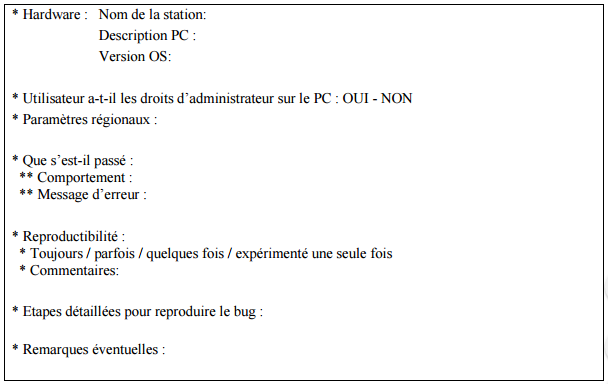
\includegraphics[width=7cm,height=6cm]{fiche_descriptive.png} &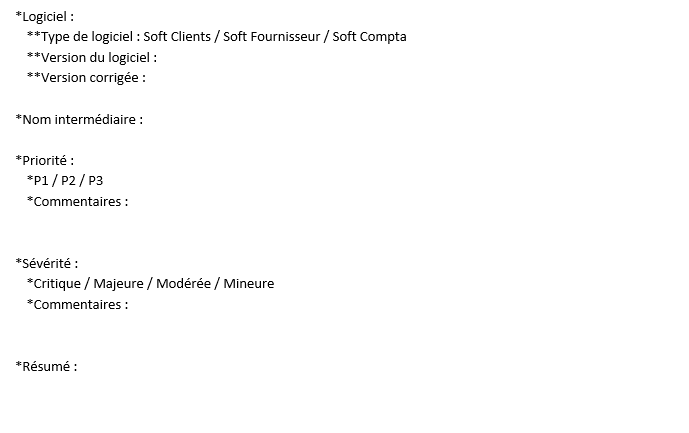
\includegraphics[width=7cm,height=6cm]{fiche_signaletique.png} \\
		\hline
	\end{tabular}
	\caption{Exemple de fiches descriptive et signalétique}
\end{table}
\label{sec:sign}
\par
Explication des différentes priorités :

\begin{itemize}
	\item \textbf{P1 :}la priorité la plus haute, réservée pour les demandes urgentes.
	\item \textbf{P2 :} la priorité moyenne.
	\item \textbf{P3 :} la priorité la plus basse.
\end{itemize}
\par
Explication des différentes sévérités :

\begin{itemize}
	\item \textbf{Critique:} la sévérité la plus haute ; elle indique que le bug est bloquant et empêche le fonctionnement du logiciel et donc la production chez les clients.
	\item \textbf{Majeure:} elle indique que le bug est grave mais qu'il existe une façon de travailler pour le contourner.
	\item \textbf{Modérée:} elle indique que le bug n'empêche pas le logiciel de fonctionner ni le client de travailler.
	\item \textbf{Mineure :} il s'agit d'un bug « cosmétique » qui sera résolu en dernier lieu.
\end{itemize}
\subsubsection{E-mail}
Par ailleurs, tous les commentaires se font actuellement via e-mail. C'est d'ailleurs via ce même e-mail que l'on suivra l'évolution du bug et que l'on gardera une trace de ce de dernier.

\subsection{Règles de gestion}

\subsubsection{Détection du bug}
Le bug est détecté / l'amélioration est demandée le plus souvent par les utilisateurs qui font parvenir cette information au commercial avec qui il est en contact. C'est le commercial qui s'occupe d'encoder le bug / l'amélioration dans le système et c'est donc ce dernier qui lance le processus de gestion.

\subsubsection{Gestion des commentaires}
Actuellement les commentaires sont gérés par e-mail. Tous les commentaires concernant un bug se rattachant au mail signalant le bug en question. De plus, l'évolution du projet se fait également via e-mail.
\subsubsection{Modification des documents}
À tout moment un membre d'équipe ou un responsable peut modifier
\hyperref[sec:sign]{ \textit{la fiche signalétique du bug}} :
\begin{itemize}
	\item le logiciel sur lequel il a rencontré le bug
	\item le nom de l'intermédiaire
	\item la version du logiciel dans laquelle le bug est survenu
	\item la version du logiciel dans laquelle le bug a été corrigé
	\item la priorité
	\item la sévérité
	\item le résumé
\end{itemize}
Il faudra donc permettre la modification de ces informations par le responsable et ses membres d'équipes. \\ \par
Par opposition, \hyperref[sec:desc]{ \textit{la fiche descriptive d'un bug}} ne pourra jamais être modifiée. Dans le cas où cette dernière serait erronée ou contiendrait une descrpition peu fiable ou devrait être tout simplement modifiée, cela se fera à l'aide de commentaires.
\subsubsection{Subdivision en différents états}
La gestion d'un bug\footnote{Nous utiliserons le mot \og bug \fg pour se référer à un bug ou à un demande d'amélioration RFE dans le reste de ce cahier des chages.} se fait à l'aide de différents états, un bug ayant toujours un état à un moment donné :
\begin{itemize}
	\item Nouveau
	\item Confirmé
	\item Pris en charge
	\item Corrigé
	\item Vérifié
	\item Clos
	\item Rejeté
	\item Non-reproductible
	\item Doublon
	\item Rouvert
\end{itemize}
Le passage d'un état à l'autre symbolise un changement dans la façon de traiter ce bug et son avancée dans le processus de résolution. Il faudra donc notifier les utilisateurs de l'évolution du projet via ces différents états.\footnote{Si un bug clos veut être rouvert, on ne changera pas l'état de ce dernier, mais on considèrera qu'il s'agit d'un nouveau bug.}
\subsubsection{Finalisation du traitement}
Seul le responsable peut décider si un bug est corrigé ou non. C'est ce dernier qui prendra la décision finale et qui mettra fin au traitement en livrant la version corrigée au client. Par ailleurs un bug pourra très bien être rouvert par la suite.


\section{Objet du marché}
La société \textit{SoftDevelop S.A.} souhaite sous-traiter le développement d'un outil de gestion des bugs
et des demandes d'améliorations, pour ses logiciels.

\subsubsection{Objectifs}
\begin{itemize}
	\item Signaler un bug ou RFE
	\item Faire évoluer le bug ou le RFE tout au long de son cycle de vie
	\item Rechercher un bug ou un RFE sur base de son identifiant unique ou de toute information de sa fiche signalétique
	\item Visualiser l'ensemble des bugs ou RFE correspondant aux critères de recherche, sous un format de tableau, chaque ligne correspondant à un bug
	\item Livrer un mode d'emploi avec l'outil de gestion des bugs
	
\end{itemize}
\subsubsection{Contraintes}
\begin{itemize}
	\item La maintenance de l'outil de gestion des bugs et des demandes d'améliorations sera assurée pendant trois ans
	\item L'application ne sera développée qu'en utilisant des standards ouverts du marché tant au
	niveau de la programmation que du langage de programmation
\end{itemize}
\newpage
\section{Spécifications applicatives}
\subsection{L'application  \textcolor{blue}{SoftRepair}\textsuperscript{TM}}
 \textcolor{red}{TO DO = INTRODUCTION}
\subsection{Description des fonctionnalités}
\begin{figure}[H]
	\centering
	\fbox{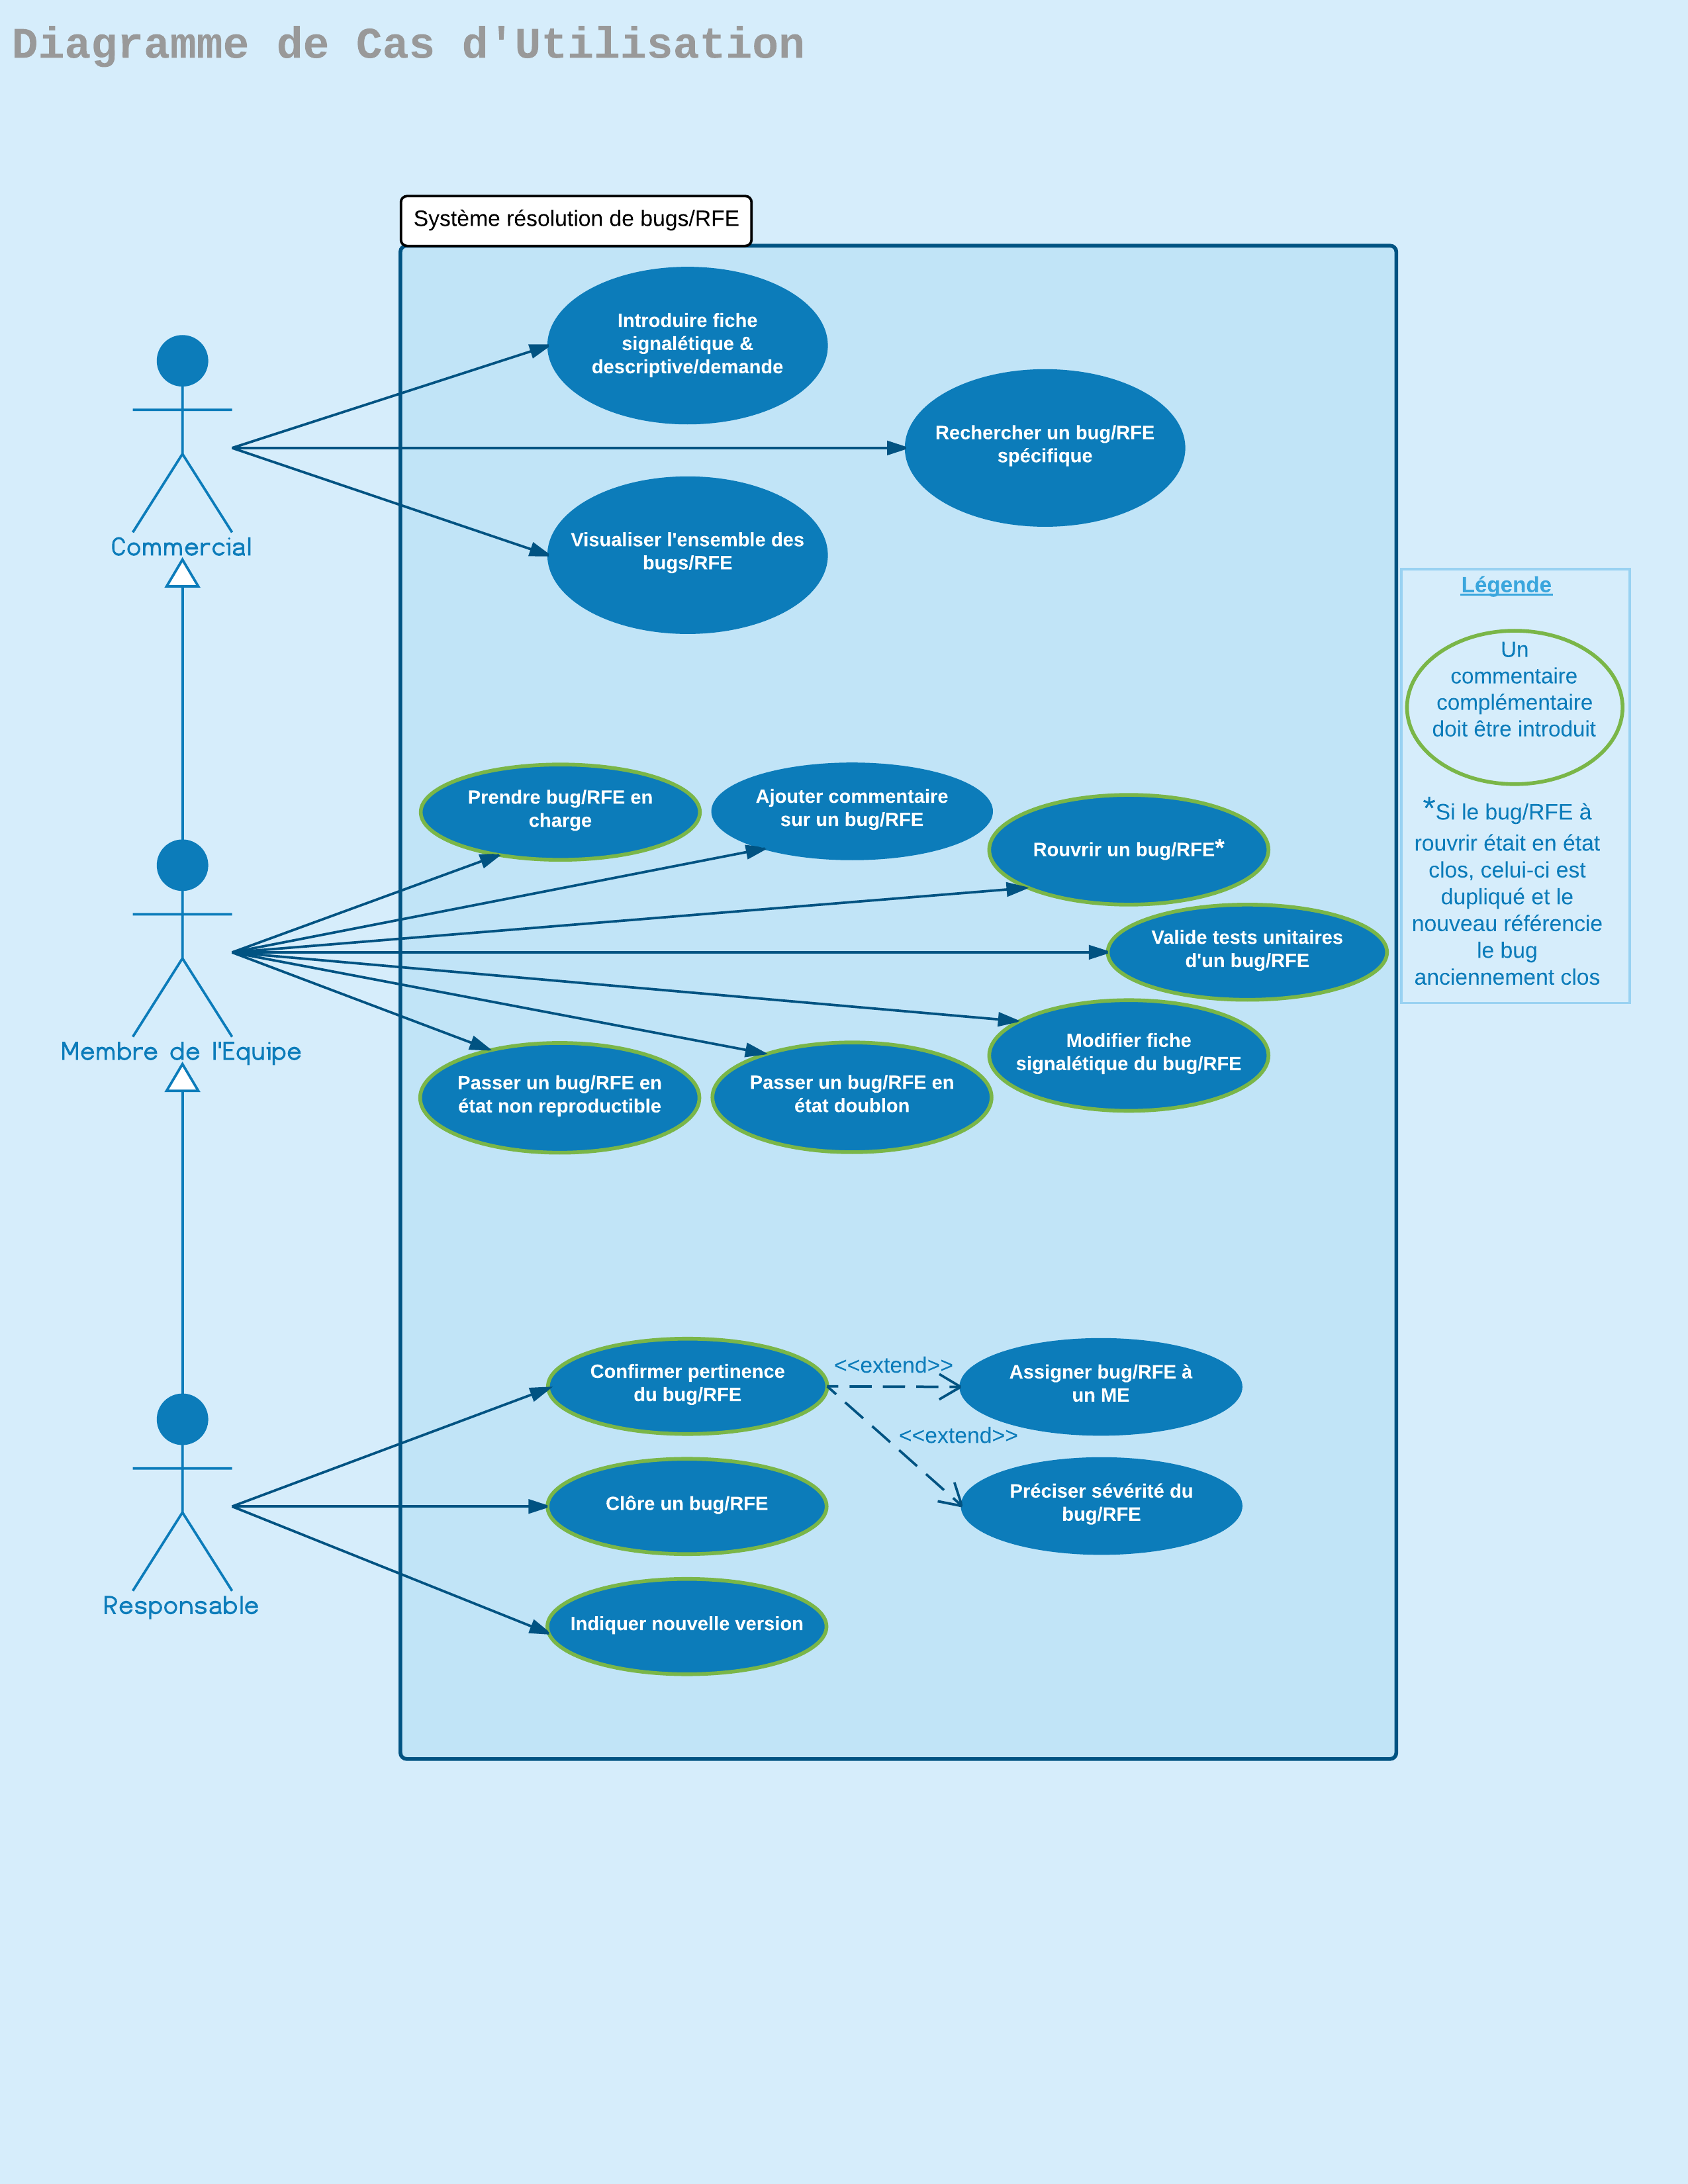
\includegraphics[width=13cm,height=14cm]{cu.png}}
	\caption{Diagramme des cas d'utilisation}
\end{figure}
\subsection{Flux d'information}
\subsubsection{Diagramme de flux d'informations}
\begin{figure}[H]
	\centering
	\fbox{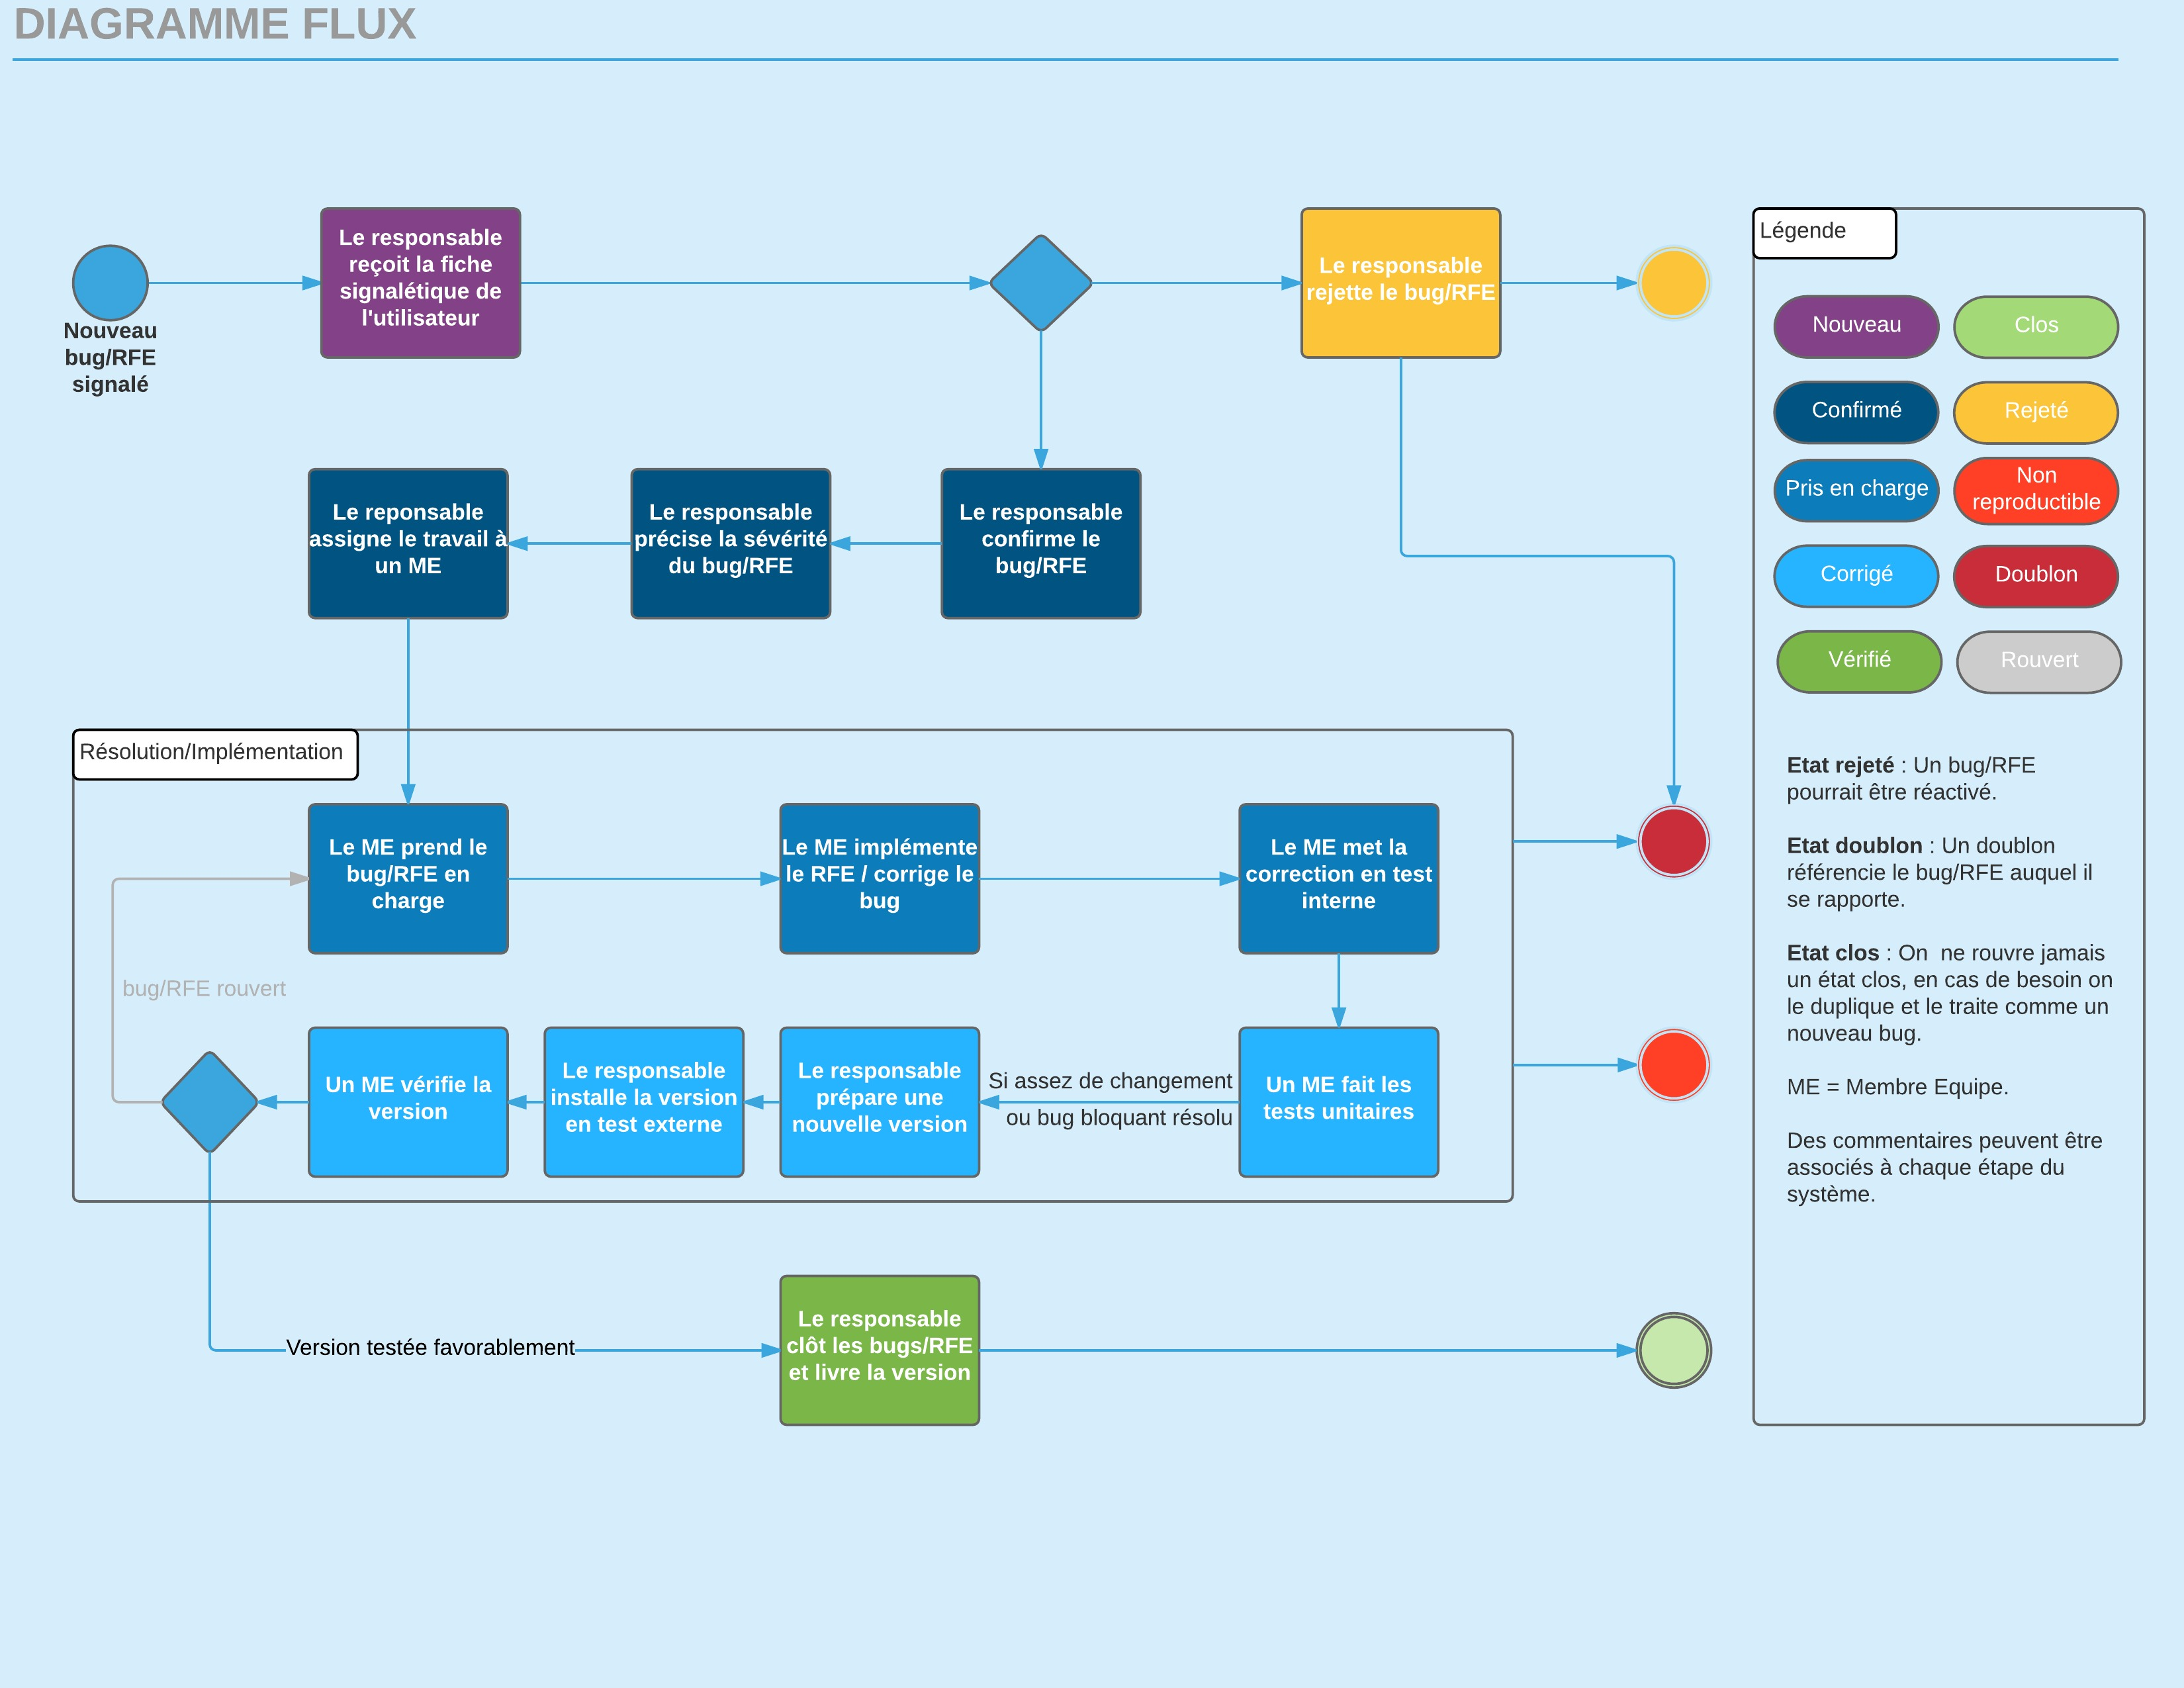
\includegraphics[width=13cm,height=14cm]{flux.jpeg}}
	\caption{Diagramme de flux de la gestion d'un bug}
\end{figure}
\subsubsection{Description du flux d'information}
Lorsqu'un nouveau bug est constaté par un intermédiaire (l'un des clients de SoftDevelop S.A.) celui-ci le fais parvenir via le commercial en remplissant une fiche signalétique ainsi qu'une fiche descriptive décrivant différents points du bug. Le responsable va par la suite vérifier sa pertinence (il répondra en outre à la question : \emph{"l'équipe va t'elle traiter ce bug / RFE"}). 
\newline
\newline
Nous distinguerons à la suite de cette étape deux cas distincts : le responsable rejette le bug / RFE et le responsable confirme le bug / RFE. Dans le cas où le bug est rejeté, ce dernier restera dans le système et pourra par la suite être réactivé. Au contraire si celui-ci est confirmé alors le responsable précisera la sévérité du bug / RFE et l'assignera à un membre de son équipe. Le membre d'équipe assigné au bug va par la suite prendre le bug en charge (on entend par là que le membre d'équipe va corriger le bug et implémenter sa solution au sein du sytème). 
\newline
\newline
Dès que le bug est corrigé, le membre d'équipe devra l'indiquer au reste de son équipe et documenter sa correction. Ensuite lorsqu'une ou plusieurs corrections de bugs doivent être livrées (Si il y a eu assez de changements pour faire une nouvelle version ou si un bug bloquant à été résolu), le responsable des développements prépare une nouvelle version et installe cette nouvelle version dans l'environnement de tests externes. Par la suite, un membre d'équipe pourra choisir un bug installé dans l'environnement de tests externes et le tester. Si le bug est testé favorablement, le membre d'équipe indique que celui-ci est vérifié et décrit les différents tests qu'il a effectué avant de parvenir à sa décision. Si au contraire un bug n'est pas 
\subsection{Description du travail des utilisateurs}
\subsubsection{L'intermédiaire}
L'intermédiaire n'est pas un utilisateur actif de l'application, sa fonction est de faire le relais entre les clients et les bugs qu'ils rencontrent et le commercial qui les signale à l'équipe de développement. Pour cela, l'application prévoit une utilsiation de suivi de bug pour que l'intermédiaire puisse informer un client de l'avancement de la résolution d'un bug en particulier. L'intermédiaire  \textbf{ n'est pas authentifié} au sein de l'application. N'importe quel utilisateur ayant accès à un bug concernant un intermédiaire peut en seul geste lui envoyer un e-mail généré automatiquement résumant l'état du bug actuel.

\textcolor{red}{NOTE : AJOUTER UNE IMAGE DU BOUTON FAIRE PART A L INTERMEDIAIRE + UN EXEMPLE DE MAIL GENERE AUTOMATIQUEMENT}

\subsubsection{Le commercial}
Le commercial est un utilisateur \textbf{authentifié} de l'application (grâce à son identifiant unique et son mot de passe). Il est le point de relais entre l'intermédiaire et l'équipe de développement, c'est lui qui signale tous nouveaux bugs. 

\paragraph{Signalement de bug}Pour cela il suit suffit depuis l'écran principal d'appuyer sur le bouton \og Ajouter un bug /RFE \fg, l'application lui invitera ensuite à remplir un formulaire correspondant à la fiche descriptive du bug.

\textcolor{red}{Note : placer ici la vue avec la fiche descriptive et signalétique d'un bug (en mettant en évidence le boutton ajouter bug) et en grisant la possibilité de changer la sévérité d'un bug}
\paragraph{Visualisation et recherche de bugs}
 Pour l'aider dans sa tâche, l'application lui permettra de visualiser l'ensemble des bugs et d'effectuer des recherches (par état, par logiciel , le concernant ou pas... \textcolor{red}{A VERIFIER/ PRECISER COHERENCE GRAPHIQUE IHM}). 
 
 \textcolor{red}{Note : placer ici la vue principal en insistant sur la partie visualistion/recherche}
 
 \paragraph{Espace personnel}
 Le commercial à également accès à son propre espace personnel depuis lequel il peut modifier ses identifiants de connexion à l'application. Depuis cet écran, il peut avoir accès à un certain nombre de statistiques le concernant. (\textcolor{red}{A VERIFIER/ PRECISER COHERENCE GRAPHIQUE IHM})


\subsubsection{Le membre d'équipe de développement}
Le membre d'équipe tient un rôle centrale dans l'application, c'est lui qui gèrera la majorité des transitions d'état des bugs afin de pouvoir garder un détail sur l'évolution de ceux-ci. Il dispose également des mêmes fonctionnalités que le commercial. La fonction de recherches de bugs possède une option supplémentaire par rapport au commercial qui lui permet de voir rapidement quels bugs lui ont été assignés par son responsable. \textcolor{red}{A VERIFIER/ PRECISER COHERENCE GRAPHIQUE IHM})
\paragraph{Insertion de commentaires}
Pour l'aider dans le développement du bug et pour tenir informer le reste de l'équipe, le membre d'équipe peut laisser un commentaire grâce à une vue prévue à cet effet. Cette action est obligatoire lorsqu'il change l'état d'un bug (un champ est directement prévu dans le menu de transition d'état pour les commentaires obligatoire ainsi que dans la fenêtre commentaires pour les facultatifs).Il est à noter que chaque commmentaire lié à un bug conserve l'état du bug durant lequel il a été écrit. La vue ci-dessous donne un exemple de l'historique des commentaires d'un bug. Un code couleur correspondant à l'état des bugs indique durant quel étape le commentaire a été écrit. 
 \textcolor{red}{Note : placer ici la vue concernant les commentaires}
\paragraph{Transition d'état}
Le menu principal du bug comprend différents boutons pour marquer la transition d'état d'un bug.

 Le membre d'équipe peut ainsi choisir de marquer un bug comme 
 
 \begin{itemize}
 	\item \textit{pris en charge} : il décide de prendre en charge son développement.
 	\item \textit{corrigé} : il considère que le bug est corrigé après avoir lui-même effectué ses tests unitaires.
 	\item \textit{validé} :il a terminé de valider les tests sur le bug en question dans l'environnement de tests de la nouvelle version (comprenant la version corrigée  du bug.
 	\item \textit{non-reproductible} :le bug est considéré comme annulé.
 	\item \textit{rouvert} : si un bug non-reproductible est remis en route.
 	\item \textit{doublon} : si le bug a déjà été signalé.
 	\item \textit{clos} : si une version reprenant le bug a déjà été livré.
 	\item \textit{nouveau} : si une version reprenant le bug a déjà été livré.
 	\item \textcolor{red}{assigné ?}
 \end{itemize}.
 \textcolor{red}{Note : placer ici la vue concernant les transitions de bug (griser celui de clore pour responsable) + monter qu'on peut bel et bien référence le bug initial pour létat doublon}
 \paragraph{Modification d'une fiche}
 Un membre d'équipe peut modifier la fiche signalétique ou descriptive d'un bug à tout moment.
  \textcolor{red}{Note : placer ici la vue où l'on peut voir un bouton pour la modification d'une fiche}
 
\subsubsection{Le responsable d'équipe de développement}
Le responsable d'équipe qui est également un utilisateur \textbf{authentifié} est doté des mêmes fonctions que le membre d'équipe. A cela près qu'il est doté d'outils supplémentaires liés aux préparation de nouvelles versions (pouvant regrouper plusieurs bugs) ainsi qu'à l'assignation de bugs à des membres d'équipes. 

\paragraph{Transitions d'états}
Trois transitions d'états lui sont réservées \og confirmé \fg et \og assigné \fg et \og clôs \fg . En effet le responsable peut dans un premier temps confirmer un nouveau bug en précisant sa sévérité mais décider de l'assigner à un membre d'équipe à un autre moment. L'état \og clôs \fg correspond à l'état d'un bug lorsque le responsable confirme la correction de celui-ci et qu'il s'apprête à préparer une nouvelle version du logiciel prenant en compte les modifications effectuées\textcolor{red}{A VERIFIER/ PRECISER COHERENCE GRAPHIQUE IHM +DSD + DIAGRAMME UC + DIAGRAMME FLUX})
  \textcolor{red}{Note : placer ici la vue où l'on peut voir le champs sévérité de la fiche signalétique non grisé + la possibilité de sélectionner un membre d'équipe pour lui assigner un bug (attention différent prise en charge, il faut rajouter un nouvel état ==> à discuter)}
\paragraph{Préparation de nouvelles versions}
Une fois qu'un ou plusieurs bugs dont l'état est \og clôs \fg le responsable peut décider de préparer une nouvelle version du logiciel concerné. Pour l'aider dans sa tâche, un  système de glisser-déposer lui permettra de reprendre les bugs repris dans la nouvelle version aisément.
  \textcolor{red}{Note : placer ici la vue où l'on prépare une nouvelle version, avec le glisser-déposer}


\subsection{Description des données}
\begin{figure}[H]
	\centering
	\fbox{\includegraphics[width=13cm,height=15cm]{dsd.png}}
	\caption{Diagramme de structures des données}
\end{figure}
\paragraph{Les utilisateurs} (commerciaux, membres d'équipe ou responsables) sont encodés dans le système par un responsable grâce à un \textit{fichier csv}. Ils s'identifient en suite dans l'application grâce çà leur identifiant personnel et leur mot de passe (hashé avec une clé BCRYPT par exemple). L'identifiant et le mot de passe peuvent ensuite être modifiés depuis l'espace personnel de chaque utilisateur.

\paragraph{Les bugs et rfes}
Les bugs qui sont en état \og corrigé \fg et qui attendent doivent être validés par un membre d'équipe sont dans une version faite par le responsable dans l'environnement de tests externes. Si le bug ne passe pas les tests à ce moment et passe en \og rouvert \fg{}, celui-ci perd également sa version puisqu'il n'est pas pas apte à permettre de passer en production. Celui-ci peut être ensuite recorrigé et revérifier mais peut être assigné à une autre version que la précédente si cette dernière est déjà mise en production.
\newline
\newline
Les bugs qui ont été corrigé par un membre d'équipe ne sont pas spécialement validés par la même personne, d'où la présence de deux relation entre bug / RFE et utilisateurs. En cas d'échec aux tests, si un bug doit être rouvert, notre application ne prévoit pas de garder un historique de toutes les personnes qui ont pris en charge et corrigé un bug, mais seulement le dernier d'entre eux. 
\newline
\newline
En cas de demande d'amélioration, seul le champs \og remarque \fg de la fiche descriptive est utilisée, c'est ce qui explique la présence de NULL (même pour le champs comportement) dans cette table.
\newline
\newline
Il est possible de référencer le doublon lié ou le bug initial en cas de bug clos que l'on souhaite rouvrir (FK bug similaire).

\paragraph{L'intermédiaire}
Il n'est pas un utilisateur de l'application, sa présence dans la base de donnée permet simplement d'envoyer rapidement un récapitulatif de l'historique d'évolution d'un bug directement par e-mail.

\paragraph{Les commentaires} jouent à la fois le rôle de commentaire d'une version ou d'un bug / RFE (c'est pourquoi le champ état est NULL notamment) Le champ \og état \fg permet de conserver l'état du bug auquel le commentaire est lié lors de son insertion dans la base de donnée.
\section{Glossaire}


 \textcolor{red}{TO DO}
\end{document}